\documentclass[12pt, twoside]{article}
\usepackage[letterpaper, margin=1in, headsep=0.5in]{geometry}
\usepackage[english]{babel}
\usepackage[utf8]{inputenc}
\usepackage{amsmath}
\usepackage{amsfonts}
\usepackage{amssymb}
\usepackage{tikz}

\usepackage{pgfplots}
\pgfplotsset{width=9cm,compat=1.9}

\usepackage{venndiagram}

\usepackage{graphicx}
\usepackage{enumitem}
\usepackage{multicol}

\usepackage{fancyhdr}
\pagestyle{fancy}
\fancyhf{}
\renewcommand{\headrulewidth}{0pt} % disable the underline of the header

\fancyhead[LE]{\thepage}
\fancyhead[RO]{\thepage \\ Name: \hspace{4cm} \,\\}
\fancyhead[LO]{BECA / Dr. Huson / IB Mathematics\\* Unit 4: Linear functions and regression\\* 13 January 2020}

\begin{document}
\begin{enumerate}
    \subsubsection*{4.8 Homework Pre-Quiz: Function operations, Linear equations}

    \item The diagram shows the straight line $L_1$, which intersects the $x$-axis at $A(6, 0)$ and the $y$-axis at $B(0,k)$. The gradient of $L_1$ is $-\frac{1}{3}$. \hfill \emph{Diagram is not to scale}
        \begin{center}
            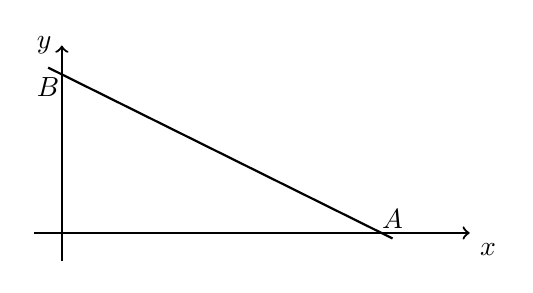
\begin{tikzpicture}[scale=.7]
            %\draw [help lines] (0,0) grid (10,8);
            \draw [thick, ->] (-0.5,0) -- (7.4,0) node [below right] {$x$};
            \draw [thick, ->] (0,-0.5)--(0,3.4) node [left] {$y$};
            %\draw [fill] (9,5) circle [radius=0.1];
            \draw [thick, -] (-0.25,3) node [below] {$B$}--(6,-0.1) node [above] {$A$};
            \end{tikzpicture}
        \end{center}
        \begin{enumerate}%[itemsep=3cm]
            \item Find the value of $k$. \hfill [2 points]
            \item Write down the equation for the line $L_1$. \hfill [2 points]
            \item The line $L_2$ is perpendicular to $L_1$ and passes through the origin. \hfill [2 points]\\[0.2cm]
            Find the equation for the line $L_2$.
        \end{enumerate}

    \item Let $f(x)=8x+3$ and $g(x)=4x$, for $x \in R$.
        \begin{enumerate}
            \item Write down  $g(2)$. \hfill [1 point]
            \item Find $(f \circ g)(x)$. \hfill [2 points]
            \item Find $f^{-1}(x)$. \hfill [2 points]
        \end{enumerate}

    \item Spicy: The diagram below shows the graph of a function $f$ for $-1 \leq x \leq 3$. 
        \begin{center}
        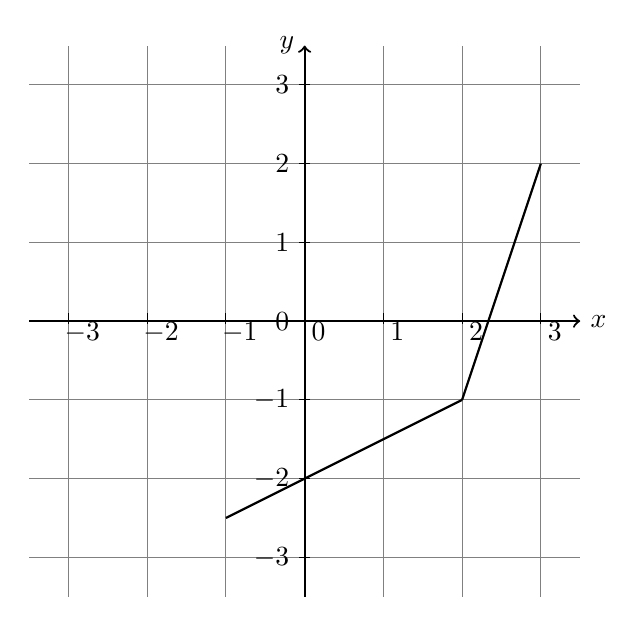
\begin{tikzpicture}[scale=1.0]
                \draw [thin, color=gray, xstep=1.0cm,ystep=1.0cm] (-3.5,-3.5) grid (3.5,3.5);
                %\draw [thin, color=lightgray,, xstep=0.2cm,ystep=0.2cm] (-5.5,-4.5) grid (5.5,6.5);
                \foreach \x in {-3, -2, -1, 0,1,2,3}
                    \draw[shift={(\x,0)},color=black] (0pt,-1pt) -- (0pt,3pt) node[below]  {$\quad \x$};
                \foreach \y in {-3, -2,-1,0,1,2,3}
                    \draw[shift={(0,\y)},color=black] (2pt,0pt) -- (-2pt,0pt) node[left]  {$\y$};
                \draw [thick, ->] (-3.5,0) -- (+3.5,0) node [right] {$x$};
                \draw [thick, ->] (0,-3.5) -- (0,3.5) node [left] {$y$};
            \draw [thick] plot[domain= -1:2] (\x, \x*1/2 -2);
            \draw [thick] (2,-1)--(3,2);
            %\draw [fill] (-3,3) circle[radius=0.1] node[above left]{$A(-3,3)$};
        \end{tikzpicture}
        \end{center}
        \begin{enumerate}%[itemsep=2cm]
            \item Write down the value of $f(2)$. \hfill [1 point]
            \item Write down the value of $f^{-1}(-2)$. \hfill [2 points]
            \item Sketch the graph of $f^{-1}$ on the grid. \hfill [3 points]
        \end{enumerate}

\newpage
\subsubsection*{Solutions} \vfill

\begin{center}
    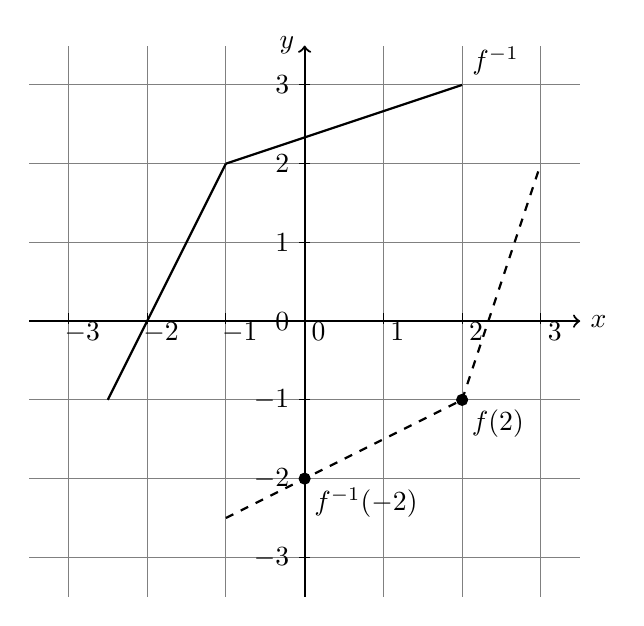
\begin{tikzpicture}[scale=1.0]
            \draw [thin, color=gray, xstep=1.0cm,ystep=1.0cm] (-3.5,-3.5) grid (3.5,3.5);
            %\draw [thin, color=lightgray,, xstep=0.2cm,ystep=0.2cm] (-5.5,-4.5) grid (5.5,6.5);
            \foreach \x in {-3, -2, -1, 0,1,2,3}
                \draw[shift={(\x,0)},color=black] (0pt,-1pt) -- (0pt,3pt) node[below]  {$\quad \x$};
            \foreach \y in {-3, -2,-1,0,1,2,3}
                \draw[shift={(0,\y)},color=black] (2pt,0pt) -- (-2pt,0pt) node[left]  {$\y$};
            \draw [thick, ->] (-3.5,0) -- (+3.5,0) node [right] {$x$};
            \draw [thick, ->] (0,-3.5) -- (0,3.5) node [left] {$y$};
        \draw [thick, dashed] plot[domain= -1:2] (\x, \x*1/2 -2);
        \draw [thick, dashed] (2,-1)--(3,2);
        \draw [thick] (-2.5,-1)--(-1,2);
        \draw [thick] (-1,2)--(2,3)node[above right]{$f^{-1}$};
        \draw [fill] (2,-1) circle[radius=0.07] node[below right]{$f(2)$};
        \draw [fill] (0,-2) circle[radius=0.07] node[below right]{$f^{-1}(-2)$};
    \end{tikzpicture}
    \end{center}

\end{enumerate}
\end{document}